\documentclass[a4paper]{article}
\usepackage{graphicx}
\usepackage[spanish,activeacute]{babel}
\usepackage{lmodern}
\usepackage{float}
\usepackage{courier}
\usepackage{multirow}
\usepackage[table,xcdraw]{xcolor}
\renewcommand{\baselinestretch}{1} % Interlineado. 1 es estandar%
\usepackage[utf8]{inputenc}
\usepackage[T1]{fontenc}
\usepackage[square,sort,comma,numbers]{natbib}
\usepackage{mathtools}
\usepackage{fancyhdr}
\fancyhead[R]{2020}\fancyhead[L]{UNC - FCEFyN} \fancyfoot[C]{\thepage}
\pagestyle{fancy}
\usepackage[numbered]{bookmark} % Para que figure las secciones en el PDF
\usepackage{xcolor}
\definecolor{vgreen}{RGB}{104,180,104}
\definecolor{vblue}{RGB}{49,49,255}
\definecolor{vorange}{RGB}{255,143,102}
\usepackage{listings}
\usepackage{trace}
\usepackage[export]{adjustbox}[2011/08/13]
%\usepackage{anysize}
%\marginsize{2cm}{2cm}{2cm}{2cm} 
\renewcommand{\lstlistingname}{Código}

\definecolor{mGreen}{rgb}{0,0.6,0}
\definecolor{mGray}{rgb}{0.5,0.5,0.5}
\definecolor{mPurple}{rgb}{0.58,0,0.82}
\definecolor{backgroundColour}{rgb}{0.95,0.95,0.92}

\lstdefinestyle{verilog-style}
{
    language=Verilog,
    basicstyle=\small\ttfamily,
    keywordstyle=\color{vblue},
    identifierstyle=\color{black},
    commentstyle=\color{vgreen},
    numbers=left,
    numberstyle=\tiny\color{black},
    numbersep=10pt,
    tabsize=8,
    moredelim=*[s][\colorIndex]{[}{]},
    literate=*{:}{:}1
}

\makeatletter
\newcommand*\@lbracket{[}
\newcommand*\@rbracket{]}
\newcommand*\@colon{:}
\newcommand*\colorIndex{%
    \edef\@temp{\the\lst@token}%
    \ifx\@temp\@lbracket \color{black}%
    \else\ifx\@temp\@rbracket \color{black}%
    \else\ifx\@temp\@colon \color{black}%
    \else \color{vorange}%
    \fi\fi\fi
}
\makeatother

\lstset{
  numbers=left,
  stepnumber=1,
  firstnumber=1,
  numberfirstline=true
}

\begin{document}
\renewcommand\tablename{Tabla}
\renewcommand\figurename{Imagen}
\begin{titlepage}
	
	{\scshape\LARGE Universidad Nacional de Córdoba \par}
	%\vspace{1cm}
	{\Large Facultad de Ciencias Exactas, Físicas y Naturales \par}
	\vspace{0.5cm}
	\centering
	
\includegraphics[width=0.5\textwidth]{unc.png}
	\par\vspace{0.5cm}
	\vspace{0.5cm}
	{\scshape\Large Arquitectura de Computadoras\par}
	\vspace{1.5cm}
	{\large\bfseries Trabajo Práctico Final \par}
	\vspace{0.2cm}
	{\normalsize \bfseries Pipeline procesador MIPS simplificado \par}
	\vspace{1.5cm}
	{\Large\bfseries COLLANTE, Gerardo\par}
	{\Large\bfseries QUINTEROS CASTILLA, Nicolás\par}
	\vfill
	Profesor:\par
	Ing. \textsc{Rodríguez}, ~Martín
	

	\vfill

% Bottom of the page
	{\large \today\par}
\end{titlepage}

%This document is an example of \texttt{natbib} package using in bibliography
%management. Three items are cited: \textit{The \LaTeX\ Companion} book 
%\cite{latexcompanion}, the Einstein journal paper \citep{einstein}, and the 
%Donald Knuth's website. The \LaTeX\ related items are 
%\citet{poole1998}. 

\tableofcontents

%\begin{lstlisting}[style={verilog-style}]
%module Mixing {
%    ///////// ADC /////////
%    inout              ADC_CS_N,
%    output             ADC_DIN,
%    input              ADC_DOUT,
%    output             ADC_SCLK,
%
%    ///////// ADC /////////
%    input              AUD_ADCDAT,
%    inout              AUD_ADCLRCK,
%    inout              AUD_BCLK,
%    output             AUD_DACDAT,
%    inout              AUD_DACLRCK,
%    output             AUD_XCK,
%
%    ///////// clocks /////////
%    input              clock2_50,
%    input              clock3_50,
%    input              clock4_50,
%    input              clock_50,
%
%    ///////// HEX /////////
%    output      [6:0]  HEX0,
%    output      [6:0]  HEX1,
%    output      [6:0]  HEX2,
%    output      [6:0]  HEX3,
%    output      [6:0]  HEX4,
%    output      [6:0]  HEX5,
%
%    ///////// FOO /////////
%    output      [2]    FOO,
%}
%\end{lstlisting}

\clearpage

\section{Introducción}
Con el nombre de MIPS (siglas de \textit{Microprocessor without Interlocked Pipeline Stages}) se conoce a toda una familia de microprocesadores de arquitectura RISC (\textit{Reduced Instruction Set Computer}) desarrollados por \textit{MIPS Technologies}.

En este trabajo práctico se solicita implementar en el lenguaje de descripción de hardware \texttt{Verilog}  (usado para modelar sistemas electrónicos usualmente) el \textit{pipeline} del procesador \textit{MIPS}.

\section{Requerimientos}
\subsection{Etapas}
Se solicita implementar las siguientes etapas del procesador:
\begin{enumerate}
	\item \texttt{IF} \textit{(Instruction Fetch)}: búsqueda de la instrucción en la memoria del programa.
	\item \texttt{ID} \textit{(Instruction Decode)}: decodificación de la instrucción y lectura de registros.
	\item \texttt{EX} \textit{(Execute)}: ejecución de la instrucción propiamente dicha.
	\item \texttt{MEM} \textit{(Memory Access)}: lectura o escritura desde/hacía la memoria de datos.
	\item \texttt{WB} \textit{(Write Back)}: escritura de resultados en los registros.
\end{enumerate}

\subsection{Instrucciones}
Se solicita implementar las siguientes instrucciones:
\begin{itemize}
	\item \texttt{R-Type}: \texttt{SLL, SRL, SRA, SLLV, SRLV, SRAV, ADDU, SUBU, AND, OR, XOR, NOR, SLT}
	\item \texttt{I-Type}: \texttt{LB, LH, LW, LWU, LBU, LHU, SB, SH, SW, ADDI, ANDI, ORI, XORI, LUI, SLQTI, BEQ, BNE, J, JAL}
	\item \texttt{J-Type}: \texttt{JR, JALR}
\end{itemize}

\subsection{Riesgos}
El procesador debe tener soporte para los siguientos tipos:
\begin{itemize}
	\item \textbf{Estructurales}: se producen cuando dos instrucciones tratan de utilizar el mismo recurso en el mismo ciclo.
	\item \textbf{Datos}: se intenta utilizar un dato antes de que esté preparado. Mantenimiento del orden estricto de lecturas y escrituras.
	\item \textbf{Control}: intentar tomar una decisión sobre una condición todavía no evaluada.
\end{itemize}

Por tanto se deberá implementar una \textbf{unidad de cortocircuitos} y una \textbf{unidad de detección de riesgos}.

\subsection{Otros}
El programa a ejecutar debe ser cargado en la memoria de programa mediante un archivo ensamblado, por tanto debe crearse un ensamblador.

\section{Ensamblador}

\section{Etapas o módulos principales}
Se realizará una breve descripción de cada una de las etapas del procesador.

\subsection{\texttt{IF}}
La etapa de \textit{Instruction Fetch} corresponde a la búsqueda de la instrucción a la memoria para posteriormente ejecutarla.

\begin{figure}[H]
	\begin{center}				
	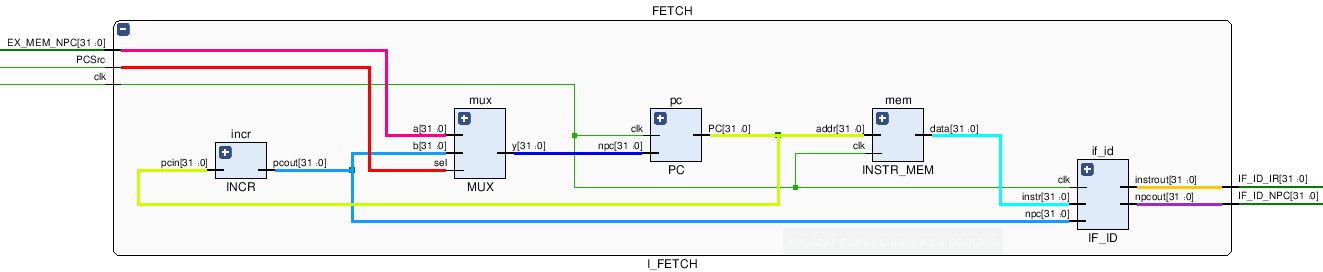
\includegraphics[width=1.4\textwidth,center]{TP4_17.png}
  	\caption{Esquemático del \textit{stage} \texttt{IF}.}
  	\label{fig:funcionamiento.}
  	\end{center}
\end{figure}

\subsubsection{\texttt{INCR}}

Incrementa el valor del \texttt{PC}.

\subsubsection{\texttt{MUX}}

Este módulo a través del selector decide cual será el próximo valor del \texttt{PC}, en función a la operación realizada en el 

\subsubsection{\texttt{PC}}
Asigna el valor al \texttt{PC}, además lo envía a \texttt{INCR} y \texttt{MEM}.

\subsubsection{\texttt{MEM}}

El módulo posee un arreglo de instrucciones que fueron cargadas previamente, entonces el \texttt{PC} sirve como índice para obtener la instrucción.

\subsubsection{\texttt{IF\_ID}}

Es el \textit{buffer} de salida, por tanto en el próximo flanco positivo de \texttt{clk}, se cargaran los valores haciendo avanzar la instrucción al siguiente \textit{stage}. Recordemos que en el momento que la instrucción se encuentra disponible en algún \textit{buffer} de salida también lo está para el siguiente \textit{stage}.

\subsubsection{Esquemático general e I/O}

\begin{figure}[H]
	\begin{center}				
	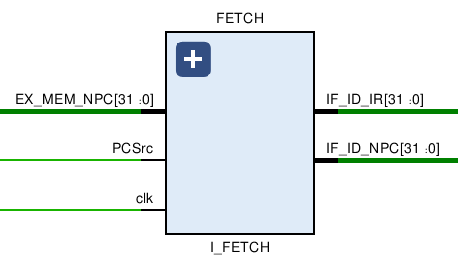
\includegraphics[width=0.40\textwidth]{TP4_1.png}
  	\caption{Módulo \texttt{IF}.}
  	\label{fig:funcionamiento.}
  	\end{center}
\end{figure}

En función al contador del programa (\texttt{PC}) se decide cual será la próxima instrucción leída desde memoria.

\textbf{Entradas}
\begin{itemize}
	\item \texttt{EX\_MEM\_NPC}: valor de \texttt{PC} obtenido desde \texttt{ADDER} (ver sección~\ref{sec:adder}) en \texttt{EX}.
	\item \texttt{PCSrc}: selector de \texttt{PC}.
\end{itemize}

\textbf{Salidas}
\begin{itemize}
	\item \texttt{IF\_ID\_IR}: instrucción.
	\item \texttt{IF\_ID\_NPC}: valor del \texttt{PC}.
\end{itemize}

\subsection{\texttt{ID}}
La etapa de \textit{Instruction Decode} corresponde a la decodificación de la instrucción.

\begin{figure}[H]
	\begin{center}				
	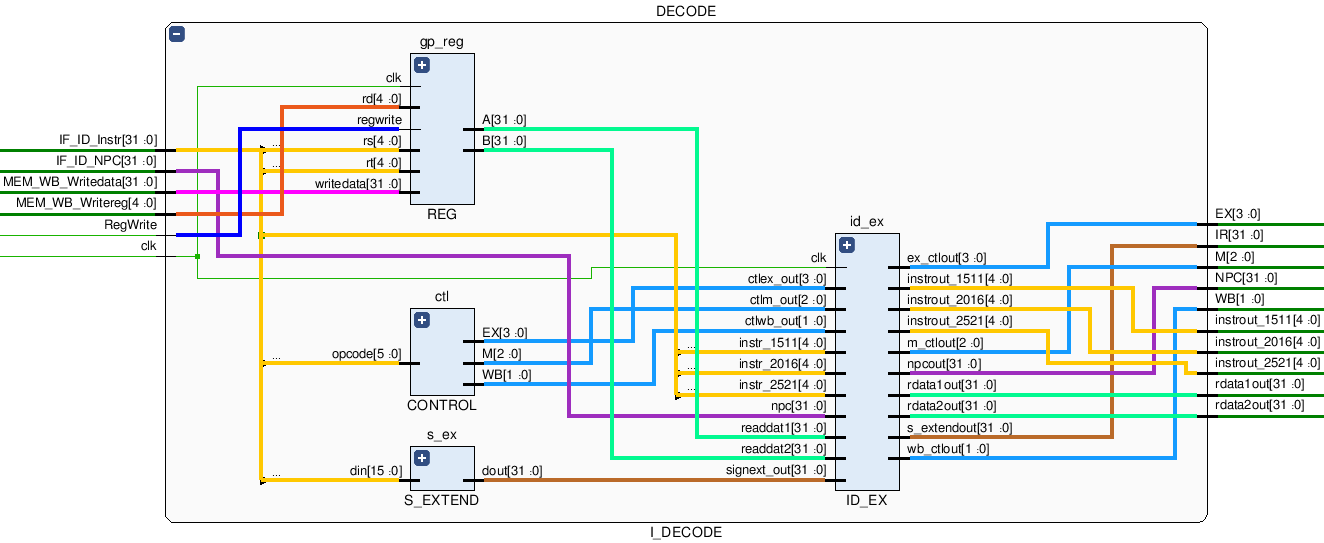
\includegraphics[width=1.4\textwidth,center]{TP4_7.png}
  	\caption{Esquemático del \textit{stage} \texttt{ID}.}
  	\label{fig:funcionamiento.}
  	\end{center}
\end{figure}

\subsubsection{\texttt{REG}}
Es el módulo encargado de almacenar los valores en lo que sería equivalente a la memoria RAM. Para ello se vale de un arreglo de 32 posiciones de 32 bits cada uno. 

Para la lectura de valores, \textit{i.e.}, \texttt{A} y \texttt{B} se indexa con \texttt{rs} y \texttt{rt} respectivamente.

Sin embargo para escribir en la memoria es necesario que \texttt{regwrite} esté en alto, y así en el \textit{rise edge} del \texttt{clk} se escribirán los datos de \texttt{writedata} en la pocisión indexada por \texttt{rd}.

\subsubsection{\texttt{CONTROL}}
Nos permite controlar los futuros \textit{stages} a través de líneas de control que serán \texttt{EX}, \texttt{M} y \texttt{WB} respectivamente, en función del \textit{opcode} de la instrucción.

Cada línea de control tiene una función especifica que se define en la siguiente Tabla~\ref{tab:ctl2-table}.

\begin{table}[H]
\centering
%\begin{tabular}{|l|l|l|}
\begin{tabular}{|p{1.6cm}|p{4.3cm}|p{4.3cm}|}
\hline
\multicolumn{1}{|c|}{\textbf{\textbf{Señal}}} &
  \multicolumn{1}{c|}{\textbf{\textbf{0}}} &
  \multicolumn{1}{c|}{\textbf{\textbf{1}}} \\ \hline
\texttt{RegDst} &
  El número de registro destino para el registro \texttt{Write} viene del campo \texttt{rd}. &
  El número de registro destino para el registro \texttt{Write} viene del campo \texttt{rt}. \\ \hline
\texttt{RegWrite} &
  Nada. &
  El registro \texttt{Write} es escrito con el valor del registro \texttt{WriteData}. \\ \hline
\texttt{ALUSrc} &
  El segundo operando de la \texttt{ALU} viene de \texttt{Read data 2}. &
  El segundo operando de la \texttt{ALU} es el \texttt{sign-extended}, los 16 bits más bajos de la instrucción. \\ \hline
\texttt{PCSrc} &
  El \texttt{PC} es reemplazado por la salida del sumador que calcula \texttt{PC+4}. &
  El \texttt{PC} es reemplazado por la salida del sumador que calcula la rama objetivo. \\ \hline
\texttt{MemRead} &
  Nada. &
  El contenido de datos de memoria indexado por la dirección de entrada es puesto en la salida de \texttt{Read Data}. \\ \hline
\texttt{MemWrite} &
  Nada. &
  El contenido de datos de memoria indexado por la dirección de entrada es reemplazado por el valor de \texttt{Write Data}. \\ \hline
\texttt{MemtoReg} &
  El valor que alimenta al registro \texttt{Write Data} viene de la \texttt{ALU}. &
  El valor que alimenta al registro \texttt{Write Data} viene desde la memoria de datos. \\ \hline
\end{tabular}
\caption{Función de cada señal de control.}
\label{tab:ctl2-table}
\end{table}

\clearpage

Básicamente consiste en la implementación de un circuito combinacional de la Tabla~\ref{tab:ctl-table}.

\begin{table}[H]

\centering
\resizebox{\textwidth}{!}{
\begin{tabular}{|l|c|c|c|c|c|c|c|c|c|c|}
\hline
\multicolumn{2}{|c|}{\multirow{2}{*}{Instruction}} &
  \multicolumn{4}{c|}{Líneas de control de la etapa de cálculo EX} &
  \multicolumn{3}{c|}{Líneas de control de etapa de acceso a MEM} &
  \multicolumn{2}{c|}{Líneas de control de la etapaWB} \\ \cline{3-11} 
\multicolumn{2}{|c|}{} & RegDst & ALUOp1 & ALUOp0 & ALUSrc & Branch & Mem-Read & Mem-Write & Reg-Write & Memto-Reg \\ \hline
R-format    & 000000   & 1      & 1      & 0      & 0      & 0      & 0        & 0         & 1         & 0         \\ \hline
lw          & 100011   & 0      & 0      & 0      & 1      & 0      & 1        & 0         & 1         & 1         \\ \hline
sw          & 101011   & x      & 0      & 0      & 1      & 0      & 0        & 1         & 0         & x         \\ \hline
beq         & 000100   & x      & 0      & 1      & 0      & 1      & 0        & 0         & 0         & x         \\ \hline
\end{tabular}}
\caption{Control de líneas}
\label{tab:ctl-table}
\end{table}

\subsubsection{\texttt{S-EXTEND}}
Incrementa el tamaño de la instrucción de 16bits a 32bits, replicando el bit de mayor orden en \texttt{[31:16]}.

\subsubsection{\texttt{ID\_EX}}
\textit{Buffer} de salida encargado de cargar los valores para la siguiente etapa, recordemos que se activa por \textit{rise edge} de \texttt{clk}.

\subsubsection{Esquemático general e I/O}
El módulo \texttt{DECODE} nos provee funcionalidades para decodificar una instrucción, leer y escribir en RAM y finalmente controlar otras etapas a través de líneas de control.

\begin{figure}[H]
	\begin{center}				
	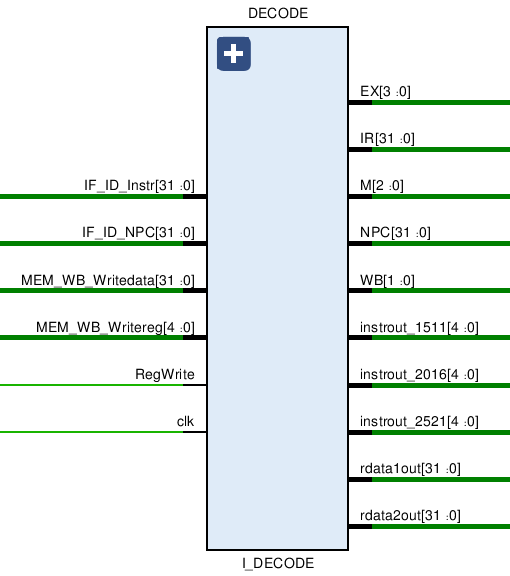
\includegraphics[width=0.32\textwidth]{TP4_3.png}
  	\caption{Módulo \texttt{ID}.}
  	\label{fig:funcionamiento.}
  	\end{center}
\end{figure}

\textbf{Entradas}
\begin{itemize}
	\item \texttt{IF\_ID\_Instr}: instrucción proveniente de \texttt{IF}.
	\item \texttt{IF\_ID\_NPC}: valor del \texttt{PC}.
	\item \texttt{MEM\_WB\_Writedata}: dato a escribir en memoria.
	\item \texttt{MEM\_WB\_Writereg}: posición donde se escribirá el dato.
	\item \texttt{RegWrite}: habilitación de escritura.
\end{itemize}

\textbf{Salidas}
\begin{itemize}
	\item \texttt{EX}, \texttt{M}, \texttt{WB}: líneas de control.
	\item \texttt{IR}: instrucción.
	\item \texttt{NPC}: valor del contador de programa.
	\item \texttt{instruot\_1511}: \texttt{rd}.
	\item \texttt{instruot\_2016}: \texttt{rt}.
	\item \texttt{instruot\_2521}: \texttt{rs}.
	\item \texttt{rdata1out}: \texttt{A}.
	\item \texttt{rdata2out}: \texttt{B}.
\end{itemize}

\subsection{\texttt{EX}}

\begin{figure}[H]
	\begin{center}				
	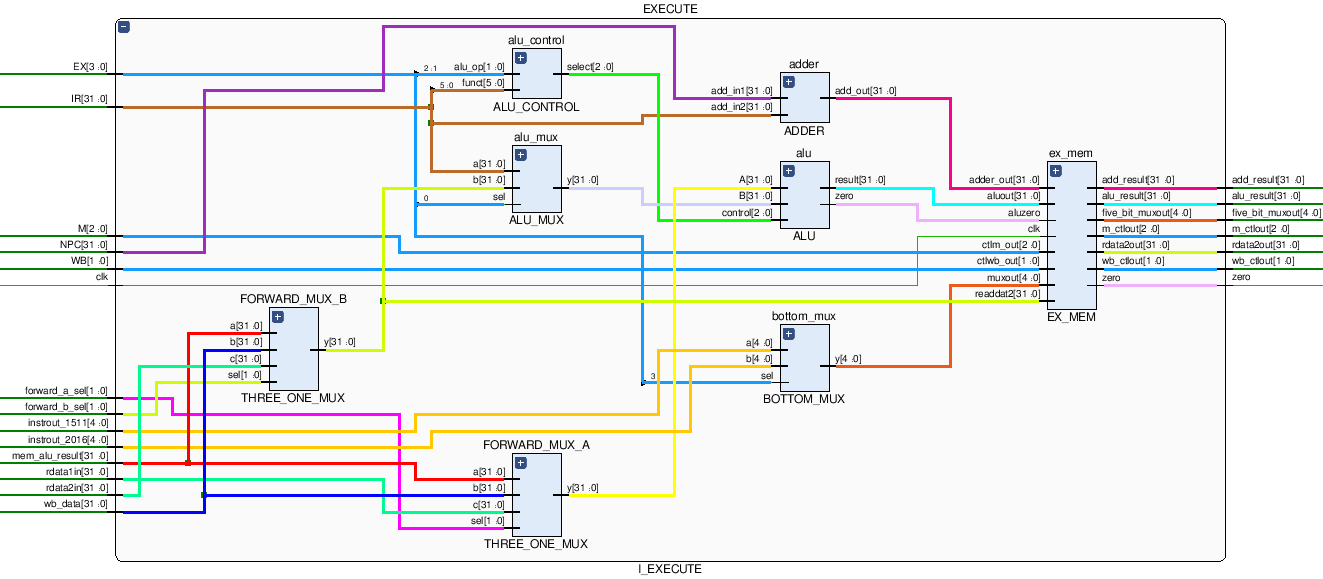
\includegraphics[width=1.5\textwidth,center]{TP4_9.png}
  	\caption{Esquemático del \textit{stage} \texttt{EX}.}
  	\label{fig:funcionamiento.}
  	\end{center}
\end{figure}

\subsubsection{\texttt{ALU\_CONTROL}}
Este módulo nos es útil para controlar la operación ejecutada por la ALU. Para esta labor utiliza \texttt{EX[2:1]} y el \textit{opcode} que equivale a \texttt{IR[31:26]}, entradas de la Tabla~\ref{tab:alu-table} a implementar.

\begin{table}[H]
\centering
\resizebox{\textwidth}{!}{
\begin{tabular}{|l|c|l|c|l|c|}
\hline
\textbf{Opcode} &
  \multicolumn{1}{l|}{\textbf{ALUOp}} &
  \textbf{Operación de la instrucción} &
  \multicolumn{1}{l|}{\textbf{Campo funct}} &
  \textbf{Acción deseada de ALU} &
  \multicolumn{1}{l|}{\textbf{Entrada de control ALU}} \\ \hline
LW           & 00 & load word        & xxxxxx & add              & 0010 \\ \hline
SW           & 00 & store word       & xxxxxx & add              & 0010 \\ \hline
Branch equal & 01 & branch equal     & xxxxxx & substract        & 0110 \\ \hline
R-type       & 10 & add              & 100000 & add              & 0010 \\ \hline
R-type       & 10 & substract        & 100010 & substract        & 0110 \\ \hline
R-type       & 10 & and              & 100100 & and              & 0000 \\ \hline
R-type       & 10 & or               & 100101 & or               & 0001 \\ \hline
R-type       & 10 & set on less than & 101010 & set on less than & 0111 \\ \hline
\end{tabular}}
\caption{Tabla de control de ALU}
\label{tab:alu-table}
\end{table}

\subsubsection{\texttt{ADDER}} \label{sec:adder}
Retorna como salida el valor actual del \texttt{PC} al de la instrucción, lo que posiblemente si se dan las condiciones sea el nuevo valor del \texttt{PC}.

\subsubsection{\texttt{ALU\_MUX}}
La \texttt{FU} (\textit{Forwarding Unit}) es la encargada de los controles de peligros así como también la encargada de decidir los valores que operará la \texttt{ALU} ya que \texttt{A} está definida por \texttt{FORWARD\_MUX\_A} y \texttt{B} si bien se define por \texttt{sel} (\texttt{EX[0]}), \texttt{b} es provisto por \texttt{FORWARD\_MUX\_B}.

Esto se explica en mayor detalle en la sección \ref{sec:fu}.

\subsubsection{\texttt{ALU}}
La \texttt{ALU} es capaz de ejecutar las operaciones de suma, resta, \texttt{and}, \texttt{or}  y si \texttt{A<B} entonces \texttt{1}, sino \texttt{0}.

Además provee un cable \texttt{zero} para las operaciones de rama.

\subsubsection{\texttt{BOTTOM\_MUX}} \label{subsubsection}
Este módulo puede consultarse en la Sección~\ref{sec:bottom}.

\subsubsection{\texttt{EX\_MEM}}
\textit{Buffer} de salida del módulo.

\subsubsection{\texttt{FORWARD\_MUX\_A}}
Consultar Tabla~\ref{tab:forwardA-table}.

\subsubsection{\texttt{FORWARD\_MUX\_B}}
Consultar Tabla~\ref{tab:forwardB-table}.

\subsubsection{Esquemático general e I/O}

\begin{figure}[H]
	\begin{center}				
	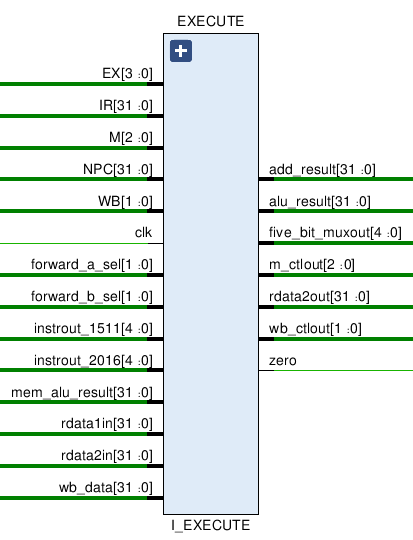
\includegraphics[width=0.4\textwidth,center]{TP4_11.png}
  	\caption{Módulo \texttt{EX}.}
  	\label{fig:funcionamiento.}
  	\end{center}
\end{figure}


\textbf{Entradas}
\begin{itemize}
	\item \texttt{EX, M, W}: líneas de control.
	\item \texttt{NPC}: valor del \texttt{PC}.
	\item \texttt{IR}: instrucción.
	\item \texttt{forward}: entradas a los multiplexores de \textit{forwarding}.
	\item \texttt{instrout\_1511}: \texttt{rd}.
	\item \texttt{instrout\_2016}: \texttt{rt}.
	\item \texttt{mem\_alu\_result}: resultado inmediato de la \texttt{ALU}.
	\item \texttt{rdata}: valores obtenidos desde \texttt{ID}.
	\item \texttt{rdata}: valor de \texttt{WB}.
		
\end{itemize}

\textbf{Salidas}
\begin{itemize}
	\item \texttt{add\_result}: resultado de \texttt{adder}.
	\item \texttt{alu\_result}: resultado inmediato de la \texttt{ALU}.
	\item \texttt{five\_bit\_muxout}: si se dan las condiciones, \texttt{rd}.
	\item \texttt{m\_cltout} y \texttt{wb\_ctlout}: líneas de control.
	\item \texttt{zero}: útil para rama.
	\item \texttt{rdata2out}: valor desde \texttt{forward\_mux\_a}.
\end{itemize}


\subsection{\texttt{FORWARDING UNIT}} \label{sec:fu}
En determinadas ocasiones en una etapa necesitamos un dato que aún no se ha terminado de procesar en otra, o quizás si pero aún el dato no ha sido guardado. Esto puede llevar a lo que se denomina parada o \textit{stall} del \textit{pipeline}, ya que necesitamos uno o más ciclos de reloj para obtener el dato. Esto acomete contra nuestro objetivo de rendimiento, por tanto necesitamos una manera de combatirlo.

Esto significa \textit{e.g.} que cuando una instrucción intenta usar un registro en su etapa \texttt{EX}, una instrucción anterior intenta escribir en su etapa \texttt{WB}, pero en realidad necesitamos los valores como entradas a la \texttt{ALU} más que en memoria.

\subsubsection{Condiciones de peligro}

\textbf{Peligro EX}

\texttt{if(EX/MEM.RegWrite and (EX/MEM.RegisterRd != 0)}

\texttt{and (EX/MEM.RegisterRd = ID/EX.RegisterRs)) ForwardA = 10}

\texttt{if(EX/MEM.RegWrite) and (EX/MEM.RegisterRd != 0)}

\texttt{and (EX/MEM.RegisterRd = ID/EX.RegisterRt)) ForwardB = 10}

\medskip

\textbf{Peligro MEM}

\texttt{if (MEM/WB.RegWrite \&\& (MEM/WB.RegisterRd !=  0)}

\texttt{\&& not(EX/MEM.RegWrite \&& (EX/MEM.RegisterRd != 0)}

\texttt{\&& (EX/MEM.RegisterRd != ID/EX.RegisterRs))}

\texttt{\&& (MEM/WB.RegisterRd = ID/EX.RegisterRs)) ForwardA = 01}

\texttt{if (MEM/WB.RegWrite \&& (MEM/WB.RegisterRd !=  0)}

\texttt{\&& not(EX/MEM.RegWrite \&& (EX/MEM.RegisterRd !=  0)}

\texttt{\&& (EX/MEM.RegisterRd !=  ID/EX.RegisterRt))}

\texttt{\&&  (MEM/WB.RegisterRd = ID/EX.RegisterRt)) ForwardB = 01}

\bigskip

Estas condiciones serán implementadas a través de dos multiplexores, \texttt{ForwardA} y \texttt{ForwardB}.

\begin{table}[H]
\centering
%\begin{tabular}{|c|c|l|}
\begin{tabular}{|c|c|p{7.5cm}|}
\hline
\texttt{ForwardA} & \textbf{Source} & \multicolumn{1}{c|}{\textbf{Primer operando de la \texttt{ALU}}}                    \\ \hline
00 & \texttt{ID/EX}  & Viene del archivo registro.                        \\ \hline
10 & \texttt{EX/MEM} & Es adelantado desde el resultado previo de la \texttt{ALU}. \\ \hline
01                & \texttt{MEM/WB}          & Es adelantado desde la memoria de datos o un resultado anterior de la \texttt{ALU} (\texttt{MemToReg} decide en \texttt{WB}). \\ \hline
\end{tabular}
\caption{Tabla del mux \texttt{ForwardA}.}
\label{tab:forwardA-table}
\end{table}

\begin{table}[H]
\centering
\begin{tabular}{|c|c|p{7.5cm}|}
\hline
\texttt{ForwardB} & \textbf{Source} & \multicolumn{1}{c|}{\textbf{Segundo operando de la \texttt{ALU}}}                   \\ \hline
00 & \texttt{ID/EX}  & Viene del archivo registro.                        \\ \hline
10 & \texttt{EX/MEM} & Es adelantado desde el resultado previo de la \texttt{ALU}. \\ \hline
01                & \texttt{MEM/WB}          & Es adelantado desde la memoria de datos o un resultado anterior de la \texttt{ALU} (\texttt{MemToReg} decide en \texttt{WB}). \\ \hline
\end{tabular}
\caption{Tabla del mux \texttt{ForwardB}.}
\label{tab:forwardB-table}
\end{table}

\subsubsection{\texttt{BOTTOM\_MUX}} \label{sec:bottom}
Este módulo es útil para obtener \texttt{rd} en el \textit{buffer} \texttt{EX\_MEM}, debido a que utiliza como selector a \texttt{EX[3]} que equivale a \texttt{RegDst}. Cuando este valor es 1, entonces selecciona \texttt{rd} como salida del multiplexor.

Esto también es beneficioso porque esta condición conlleva que \texttt{Reg-Write} este habilitado por tanto se escribirá, como observamos en la Tabla~\ref{tab:ctl-table}.

\subsubsection{Esquemático general e I/O}

\begin{figure}[H]
	\begin{center}				
	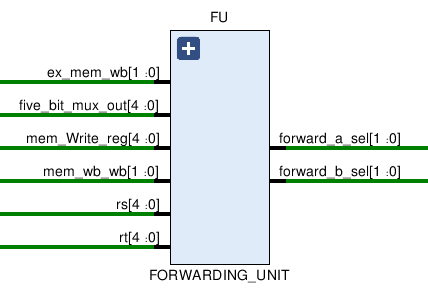
\includegraphics[width=0.5\textwidth,center]{TP4_10.png}
  	\caption{Esquemático del módulo \texttt{FU}.}
  	\label{fig:funcionamiento.}
  	\end{center}
\end{figure}

\textbf{Entradas}

\begin{itemize}
	\item \texttt{ex\_mem\_wb[1] = EX/MEM.RegWrite}
	\item \texttt{five\_bit\_mux\_out = EX/MEM.RegisterRd}
	\item \texttt{mem\_Write\_reg = MEM/WB.RegisterRd}
	\item \texttt{mem\_wb\_wb[1] = MEM/WB.RegWrite}
	\item \texttt{rs = ID/EX.RegisterRs}
	\item \texttt{rt = ID/EX.RegisterRt}
\end{itemize}

\textbf{Salidas}: las respectivas entradas a cada uno de los multiplexores ubicados en el \textit{stage} \texttt{EX}.

\begin{itemize}
	\item \texttt{forward\_a\_sel}
	\item \texttt{forward\_b\_sel} 
\end{itemize}

\subsection{\texttt{MEM}}

\begin{figure}[H]
	\begin{center}				
	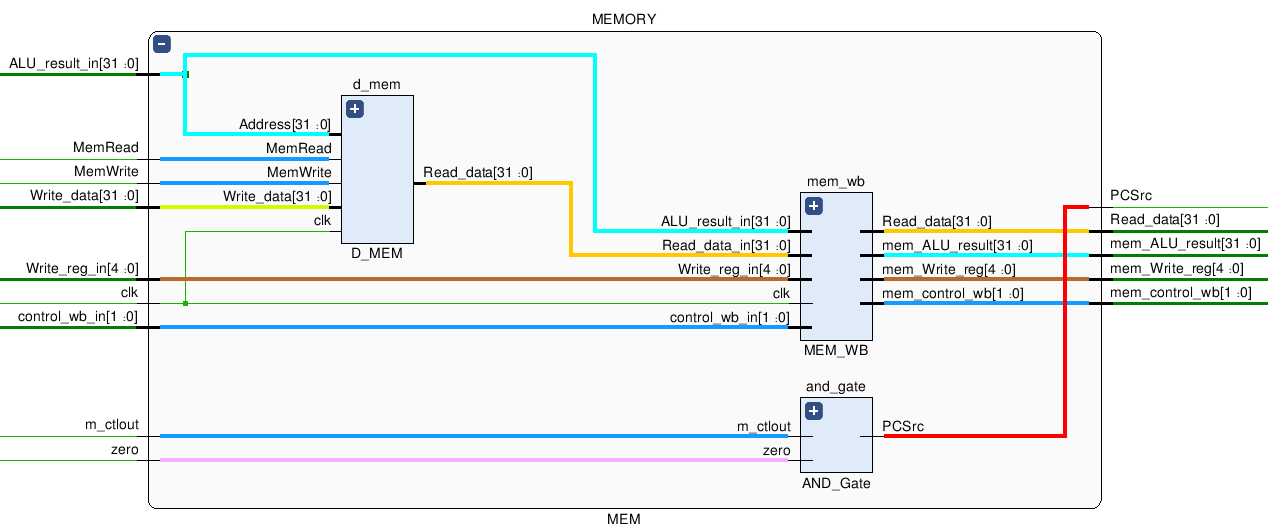
\includegraphics[width=1.5\textwidth,center]{TP4_13.png}
  	\caption{Esquemático del \textit{stage} \texttt{MEM}.}
  	\label{fig:funcionamiento.}
  	\end{center}
\end{figure}

\subsubsection{\texttt{D\_MEM}}
Equivale a la memoria ROM, posee un arreglo de 128 posiciones de 32 bits cada una.

Su funcionamiento es sencillo, \texttt{Address} funciona como índice del arreglo y tanto para leer como para escribir debemos setear los valores \texttt{MemWrite} como \texttt{MemRead} respectivamente como vimos en la Tabla~\ref{tab:ctl2-table}.

\subsubsection{\texttt{MEM\_WB}}
\textit{Buffer} de salida del \textit{stage}.

\subsubsection{\texttt{AND\_Gate}}
Realiza la operación \texttt{M[2]\&\&zero}, (recordemos que \texttt{M[2]} es \textit{branch} en la Tabla~\ref{tab:ctl-table}) obteniendo la salida \texttt{PCSrc} que luego será útil para decidir en el mux de \texttt{IF} cúal será el próximo \texttt{PC}.

\subsubsection{Esquemático general e I/O}

\begin{figure}[H]
	\begin{center}				
	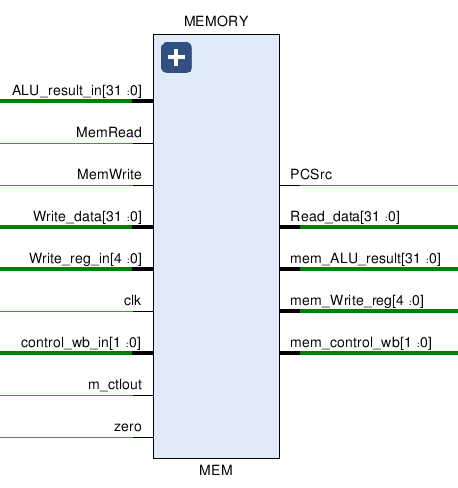
\includegraphics[width=0.5\textwidth,center]{TP4_14.png}
  	\caption{Módulo \texttt{MEM}.}
  	\label{fig:funcionamiento.}
  	\end{center}
\end{figure}

\textbf{Entradas}
\begin{itemize}
	\item \texttt{ALU\_result\_in}: resultado de la \texttt{ALU}.
	\item \texttt{MemRead}: \texttt{M[1]}.
	\item \texttt{MemWrite}: \texttt{M[0]}.
	\item \texttt{Write\_Data}: \texttt{rdata2out}.
	\item \texttt{Write\_reg\_in}: \texttt{rd} (\texttt{EX[3]=1}) o \texttt{rt}.
	\item \texttt{control\_wb\_in}: línea de control.
	\item \texttt{m\_ctlout}: \texttt{M[2]}.
	\item \texttt{zero}: proviene desde la \texttt{ALU}.
\end{itemize}

\textbf{Salidas}
\begin{itemize}
	\item \texttt{PCSrc}: selector de mux en \texttt{IF}.
	\item \texttt{Read\_data}: datos leídos.
	\item \texttt{mem\_ALU\_results} = \texttt{ALU\_result\_in}
	\item \texttt{mem\_Write\_reg} = \texttt{Write\_reg\_in}
	\item \texttt{mem\_control\_wb} = \texttt{control\_wb\_in}
\end{itemize}

\subsection{\texttt{WB}}

\begin{figure}[H]
	\begin{center}				
	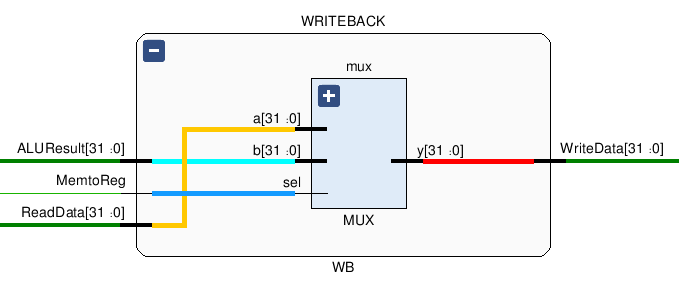
\includegraphics[width=0.9\textwidth,center]{TP4_15.png}
  	\caption{Esquemático del \textit{stage} \texttt{WB}.}
  	\label{fig:funcionamiento.}
  	\end{center}
\end{figure}

El funcionamiento de este módulo es muy simple, básicamente decide a través del selector \texttt{MemtoReg} (Tabla~\ref{tab:ctl2-table}) si \texttt{WriteData} será el valor leído desde memoria o el resultado de la \texttt{ALU}.

\subsubsection{Esquemático general e I/O}

\begin{figure}[H]
	\begin{center}				
	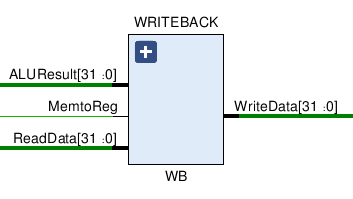
\includegraphics[width=0.5\textwidth,center]{TP4_16.png}
  	\caption{Módulo \texttt{WB}.}
  	\label{fig:funcionamiento.}
  	\end{center}
\end{figure}

\textbf{Entradas}
\begin{itemize}
	\item \texttt{ALUResult}: resultado de la \texttt{ALU}.
	\item \texttt{MemtoReg}: \texttt{mem\_control\_wb[0]}.
	\item \texttt{ReadData}: datos desde la memoria.
\end{itemize}

\textbf{Salidas}
\begin{itemize}
	\item \texttt{WriteData}: datos para \texttt{ID} y \texttt{EX}.
\end{itemize}

\section{Conclusiones}

\texttt{NAQV}

El trabajo en si mismo no presentaba una dificultad demasiado alta, sin embargo su desarrollo fue retrasado debía a que determinados pasos requerían modificaciones del \textit{linker} o agregar determinadas librerías que no estaban en el proyecto en un primer momento. Pero una vez que se sorteados estos obstáculos el desarrollo fue mucho más veloz.

Fue una grata experiencia para adquirir roce con el desarrollo de sistemas operativos de tiempo real, se comprobó su funcionamiento y su potencial para las áreas para la cual ha sido desarrollada esta tecnología.

\section{Apéndices}

\subsection{Modo de uso}

\subsubsection{Compilación}
Para compilar el proyecto es necesario abrir la consola en el directorio 

\texttt{so2-tp4-rtos-GeraCollante} y ejecutar el comando \texttt{make}.

\subsubsection{Clean}
\texttt{make clean}

\subsubsection{Ejecución}
\texttt{qemu-system-arm -machine lm3s811evb -cpu cortex-m3 -kernel gcc/RTOSDemo.axf --serial stdio}

\clearpage

\nocite{*}

\end{document}